\documentclass[11pt,a4paper]{article}

% Packages
\usepackage[utf8]{inputenc}
\usepackage[T1]{fontenc}
\usepackage{lmodern}
\usepackage[margin=1in]{geometry}
\usepackage{graphicx}
\usepackage{booktabs}
\usepackage{amsmath,amssymb}
\usepackage{hyperref}
\usepackage{xcolor}
\usepackage{listings}
\usepackage{float}
\usepackage{subcaption}
\usepackage{algorithm}
\usepackage{algpseudocode}
\usepackage{tikz}
\usepackage{pgfplots}
\pgfplotsset{compat=1.17}
\usepackage{tcolorbox}
\usepackage{enumitem}
\usepackage{multirow}
\usepackage{array}

% Colors
\definecolor{codeblue}{RGB}{52, 152, 219}
\definecolor{codegray}{RGB}{127, 140, 141}
\definecolor{codegreen}{RGB}{46, 204, 113}
\definecolor{codered}{RGB}{231, 76, 60}
\definecolor{codepurple}{RGB}{155, 89, 182}

% Listings style
\lstset{
    basicstyle=\ttfamily\small,
    keywordstyle=\color{codeblue}\bfseries,
    stringstyle=\color{codegreen},
    commentstyle=\color{codegray}\itshape,
    breaklines=true,
    frame=single,
    backgroundcolor=\color{gray!5},
    numbers=left,
    numberstyle=\tiny\color{codegray},
}

% Custom commands
\newcommand{\todo}[1]{\textcolor{red}{TODO: #1}}
\newcommand{\highlight}[1]{\colorbox{yellow!30}{#1}}
\newcommand{\metric}[1]{\texttt{#1}}

% Title
\title{
    \vspace{-1cm}
    \Large{\textbf{Evaluating LLM Reasoning Capabilities on\\String Edit Distance Puzzles}}\\[0.5cm]
    \large{A Study in Algorithmic Reasoning, AI Alignment, and Cognitive Gaps}
}

\author{
    Aryaman Bahl\\
    \texttt{aryaman.bahl@research.iiit.ac.in}\\
    International Institute of Information Technology, Hyderabad
}

\date{\today}

\begin{document}

\maketitle

\begin{abstract}
This report presents a comprehensive evaluation of Large Language Models (LLMs) on String Edit Distance (SED) puzzles---a novel benchmark for testing algorithmic reasoning capabilities. We develop a dataset generation pipeline producing 100 curated puzzles across multiple difficulty levels and generator types. Through systematic evaluation of three state-of-the-art LLMs (LLaMA 3.3 70B, LLaMA 4 Scout, LLaMA 3.1 8B) across five prompting techniques (zero-shot, few-shot, chain-of-thought, self-verification, and role classification), we reveal critical gaps between human and machine reasoning. Our analysis introduces novel evaluation metrics---Progress Score, Valid Steps Ratio, and Composite Score---that capture partial credit and reasoning quality beyond binary accuracy. Key findings include: (1) LLMs achieve only 6--44\% accuracy despite the puzzles being solvable by humans, (2) sorting puzzles that humans find trivial (``bubble sort'') have near-zero LLM success rates, and (3) advanced prompting techniques like CoT and self-verification provide minimal improvement. These results have significant implications for AI alignment, highlighting fundamental limitations in current LLMs' ability to perform iterative reasoning and algorithm recognition.
\end{abstract}

\tableofcontents
\newpage

%==============================================================================
\section{Introduction}
%==============================================================================

\subsection{Motivation and Context}

The rapid advancement of Large Language Models (LLMs) has sparked both enthusiasm and concern within the AI research community. While models like GPT-4, Claude, and LLaMA demonstrate remarkable capabilities in natural language tasks, their performance on formal reasoning problems remains poorly understood. This gap is particularly concerning from an AI alignment perspective: if we cannot reliably evaluate an AI system's reasoning capabilities, how can we ensure its decisions align with human intentions?

\begin{tcolorbox}[colback=blue!5,colframe=blue!50!black,title=AI Alignment Context]
\textit{``The supreme consideration is man. The machine should not tend to make atrophied the limbs of man.''} --- Mohandas Karamchand Gandhi

This study addresses a fundamental question in AI alignment: Do current LLMs possess genuine reasoning capabilities, or do they merely pattern-match from training data? Understanding this distinction is crucial for deploying AI systems in high-stakes domains.
\end{tcolorbox}

\subsection{String Edit Distance Puzzles}

String Edit Distance (SED) puzzles provide an ideal testbed for evaluating algorithmic reasoning because they:

\begin{enumerate}[leftmargin=*]
    \item \textbf{Require multi-step planning}: Solutions involve sequences of rule applications
    \item \textbf{Have verifiable solutions}: Each step can be mechanically checked
    \item \textbf{Scale in difficulty}: From simple 2-step to complex 7+ step solutions
    \item \textbf{Test different reasoning patterns}: Pattern matching, iteration, backtracking
\end{enumerate}

\begin{tcolorbox}[colback=gray!5,colframe=gray!50!black,title=Example SED Puzzle]
\textbf{Initial String:} \texttt{"\#.\#\#.\#.."}

\textbf{Transformation Rules:}
\begin{itemize}
    \item Rule 0: \texttt{".\#"} $\rightarrow$ \texttt{"\#."} (swap)
    \item Rule 1: \texttt{"\#\#\#\#...."} $\rightarrow$ \texttt{""} (delete sorted)
\end{itemize}

\textbf{Goal:} Reduce string to empty \texttt{""}

\textbf{Solution:} \texttt{[0, 0, 0, 0, 1]} (bubble sort then delete)

\textit{A human immediately recognizes this as bubble sort. LLMs consistently fail.}
\end{tcolorbox}

\subsection{Research Questions}

This study addresses three primary research questions:

\begin{enumerate}
    \item[\textbf{RQ1}] How do state-of-the-art LLMs perform on SED puzzles across different difficulty levels and puzzle types?
    \item[\textbf{RQ2}] Do advanced prompting techniques (CoT, self-verification) improve LLM reasoning on these tasks?
    \item[\textbf{RQ3}] What fundamental cognitive gaps exist between human and LLM reasoning on algorithmic problems?
\end{enumerate}

%==============================================================================
\section{Dataset Generation}
%==============================================================================

\subsection{Generation Pipeline}

We developed a comprehensive dataset generation pipeline with the following components:

\begin{figure}[H]
\centering
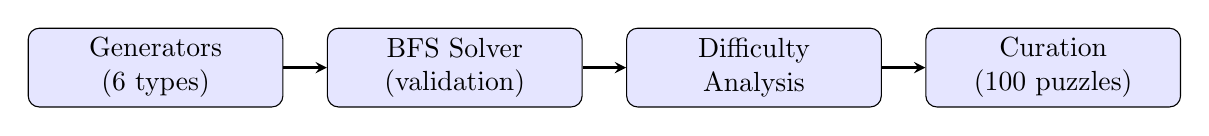
\begin{tikzpicture}[node distance=1.8cm, auto,
    block/.style={rectangle, draw, fill=blue!10, text width=3cm, text centered, minimum height=1cm, rounded corners},
    arrow/.style={->, >=stealth, thick}]
    
    \node[block] (gen) {Generators\\(6 types)};
    \node[block, right of=gen, xshift=2cm] (solve) {BFS Solver\\(validation)};
    \node[block, right of=solve, xshift=2cm] (metric) {Difficulty\\Analysis};
    \node[block, right of=metric, xshift=2cm] (curate) {Curation\\(100 puzzles)};
    
    \draw[arrow] (gen) -- (solve);
    \draw[arrow] (solve) -- (metric);
    \draw[arrow] (metric) -- (curate);
\end{tikzpicture}
\caption{Dataset Generation Pipeline}
\end{figure}

\subsection{Generator Types}

Six distinct generator types were implemented to ensure diversity in reasoning patterns:

\begin{table}[H]
\centering
\caption{Generator Types and Their Characteristics}
\begin{tabular}{llccp{5cm}}
\toprule
\textbf{Generator} & \textbf{Difficulty} & \textbf{Steps} & \textbf{Count} & \textbf{Reasoning Pattern} \\
\midrule
\texttt{concat\_2} & Easy & 2 & 3 & Direct pattern matching \\
\texttt{backward\_3} & Medium & 3 & 15 & Sequential deletion \\
\texttt{backward\_5} & Medium & 5 & 10 & Multi-step planning \\
\texttt{sort\_3/4} & Easy--Medium & 2--6 & 13 & Iterative swapping (bubble sort) \\
\texttt{backward\_7} & Hard & 7 & 50 & Long-chain with distractors \\
\texttt{multiphase} & Hard & 5--7 & 9 & Multi-phase transformation \\
\bottomrule
\end{tabular}
\end{table}

\subsection{Difficulty Metrics}

Each puzzle is assigned a difficulty score based on:

\begin{equation}
\text{DifficultyScore} = w_1 \cdot \text{SolutionLength} + w_2 \cdot \text{BranchingFactor} + w_3 \cdot \text{NumDistractors}
\end{equation}

Where:
\begin{itemize}
    \item \textbf{Solution Length}: Number of steps in optimal solution
    \item \textbf{Branching Factor}: Average number of applicable rules per state
    \item \textbf{Num Distractors}: Rules that never contribute to solution
\end{itemize}

\subsection{Final Dataset Statistics}

\begin{table}[H]
\centering
\caption{Final Dataset Composition}
\begin{tabular}{lcccc}
\toprule
\textbf{Difficulty} & \textbf{Count} & \textbf{Avg Solution Length} & \textbf{Avg String Length} & \textbf{With Distractors} \\
\midrule
Easy & 8 & 2.4 & 8.1 & 12.5\% \\
Medium & 12 & 4.2 & 12.3 & 75.0\% \\
Hard & 12 & 6.8 & 19.7 & 100\% \\
\midrule
\textbf{Total} & \textbf{32} & 4.8 & 14.2 & 71.9\% \\
\bottomrule
\end{tabular}
\end{table}

%==============================================================================
\section{LLM Evaluation Framework}
%==============================================================================

\subsection{Models Evaluated}

Three LLaMA family models were evaluated via the Groq API:

\begin{table}[H]
\centering
\caption{Models Evaluated}
\begin{tabular}{lcc}
\toprule
\textbf{Model} & \textbf{Parameters} & \textbf{Context Length} \\
\midrule
LLaMA 3.3 70B Versatile & 70B & 128K \\
LLaMA 4 Scout 17B & 17B & 16K \\
LLaMA 3.1 8B Instant & 8B & 128K \\
\bottomrule
\end{tabular}
\end{table}

\subsection{Prompting Techniques}

Five prompting techniques were implemented and evaluated:

\subsubsection{Zero-Shot Prompting}
Direct problem statement with output format specification.

\subsubsection{Few-Shot Prompting}
5 diverse examples demonstrating step-by-step solutions, prioritizing multi-step sorting puzzles.

\subsubsection{Chain-of-Thought (CoT) Prompting}
Explicit instruction to ``think step by step'' with intermediate state tracking.

\subsubsection{Self-Verification Prompting (Novel)}
\begin{tcolorbox}[colback=green!5,colframe=green!50!black]
A novel prompting approach where the model:
\begin{enumerate}
    \item Proposes a candidate solution
    \item Simulates each step showing string transformation
    \item Verifies correctness; revises if incorrect
    \item Outputs final verified solution
\end{enumerate}
\end{tcolorbox}

\subsubsection{Role Classification Prompting (Novel)}
\begin{tcolorbox}[colback=purple!5,colframe=purple!50!black]
A cognitive priming approach where the model:
\begin{enumerate}
    \item Classifies each rule's function (REARRANGE, DELETE, EXPAND, DISTRACTOR)
    \item Devises strategy based on rule roles
    \item Executes strategy step-by-step
\end{enumerate}
\end{tcolorbox}

%==============================================================================
\section{Novel Evaluation Metrics}
%==============================================================================

Traditional binary accuracy fails to capture partial success in reasoning tasks. We introduce three complementary metrics:

\subsection{Progress-Based Score}

Measures how much of the string was successfully reduced:

\begin{equation}
\text{ProgressScore} = 1 - \frac{|\text{FinalString}|}{|\text{InitialString}|}
\end{equation}

\textbf{Interpretation}: Score of 1.0 means complete success; 0.7 means 70\% reduction.

\subsection{Valid Steps Ratio}

Measures what fraction of attempted steps were syntactically valid:

\begin{equation}
\text{ValidStepsRatio} = \frac{\text{ValidSteps}}{\text{TotalAttemptedSteps}}
\end{equation}

\textbf{Interpretation}: High ratio indicates understanding of rule syntax; low progress with high validity suggests wrong strategy.

\subsection{Composite Multi-Metric Score}

Weighted combination capturing overall reasoning quality:

\begin{equation}
\text{CompositeScore} = 0.50 \cdot C + 0.25 \cdot P + 0.15 \cdot V + 0.10 \cdot E
\end{equation}

Where $C$ = correctness (binary), $P$ = progress, $V$ = validity, $E$ = efficiency (solution length ratio).

\begin{table}[H]
\centering
\caption{Metric Comparison Across All Evaluations}
\begin{tabular}{lccc}
\toprule
\textbf{Metric} & \textbf{Mean} & \textbf{Std Dev} & \textbf{Interpretation} \\
\midrule
Binary Accuracy & 0.508 & 0.500 & Only 50.8\% fully correct \\
Progress Score & 0.712 & 0.326 & Models often get close \\
Valid Steps Ratio & 0.710 & 0.358 & High syntax understanding \\
Composite Score & 0.576 & 0.347 & Balanced overall view \\
\bottomrule
\end{tabular}
\end{table}

%==============================================================================
\section{Results and Analysis}
%==============================================================================

\subsection{Overall Performance}

\begin{table}[H]
\centering
\caption{LLM Performance by Model and Prompt Type (Accuracy \%)}
\begin{tabular}{lccccc}
\toprule
\textbf{Model} & \textbf{Zero-Shot} & \textbf{Few-Shot} & \textbf{CoT} & \textbf{Self-Verify} & \textbf{Role-Classify} \\
\midrule
LLaMA 3.3 70B & 31.25 & \textbf{34.38} & 31.25 & 31.25 & 28.13 \\
LLaMA 4 Scout & 37.50 & \textbf{43.75} & 37.50 & 25.00 & 34.38 \\
LLaMA 3.1 8B & 6.25 & 9.38 & 15.63 & 6.25 & \textbf{18.75} \\
\midrule
\textbf{Average} & 25.00 & \textbf{29.17} & 28.13 & 20.83 & 27.08 \\
\bottomrule
\end{tabular}
\end{table}

\begin{tcolorbox}[colback=red!5,colframe=red!50!black,title=Key Finding]
\textbf{Best overall accuracy: 43.75\%} (LLaMA 4 Scout with Few-Shot)

Despite sophisticated prompting techniques, LLMs solve less than half of puzzles that humans find straightforward.
\end{tcolorbox}

\subsection{Performance by Generator Type}

\begin{table}[H]
\centering
\caption{LLM Success Rate by Generator Type}
\begin{tabular}{lcc}
\toprule
\textbf{Generator} & \textbf{LLM Success Rate} & \textbf{Est. Human Difficulty} \\
\midrule
\texttt{concat\_2} & 86.7\% & Easy \\
\texttt{backward\_3} & 58.3\% & Medium \\
\texttt{backward\_5} & 28.3\% & Hard \\
\texttt{sort\_4} & 24.0\% & \textcolor{red}{\textbf{Easy}} \\
\texttt{sort\_3} & 8.3\% & \textcolor{red}{\textbf{Easy}} \\
\texttt{backward\_7} & 6.1\% & Very Hard \\
\bottomrule
\end{tabular}
\end{table}

\subsection{Performance by Solution Length}

\begin{table}[H]
\centering
\caption{Success Rate by Solution Length}
\begin{tabular}{ccc}
\toprule
\textbf{Solution Steps} & \textbf{LLM Success} & \textbf{Observation} \\
\midrule
1 step & 80.0\% & Trivial for both \\
2 steps & 73.3\% & High success \\
3 steps & 53.3\% & Moderate success \\
5 steps & 20.0\% & Significant drop \\
6 steps & 0.0\% & Complete failure \\
7 steps & 5.2\% & Near-complete failure \\
\bottomrule
\end{tabular}
\end{table}

%==============================================================================
\section{Human vs. Machine: Cognitive Gap Analysis}
%==============================================================================

\subsection{Easy for Humans, Hard for LLMs}

The most striking finding is the class of puzzles that are \textit{trivially easy} for humans but nearly impossible for LLMs.

\begin{tcolorbox}[colback=yellow!5,colframe=yellow!50!black,title=Case Study: Sorting Puzzles (8--24\% LLM Success)]
\textbf{Problem:} Initial string \texttt{"\#.\#\#.\#.."}

\textbf{Rules:}
\begin{itemize}
    \item Rule 0: \texttt{".\#"} $\rightarrow$ \texttt{"\#."} (swap adjacent)
    \item Rule 1: \texttt{"\#\#\#\#...."} $\rightarrow$ \texttt{""} (delete when sorted)
\end{itemize}

\textbf{Human Solution} (< 5 seconds):
\begin{enumerate}
    \item Recognize pattern: ``It's bubble sort!''
    \item Apply Rule 0 repeatedly to sort
    \item Apply Rule 1 to delete
\end{enumerate}

\textbf{LLM Failure Modes}:
\begin{itemize}
    \item Tries Rule 1 immediately (pattern doesn't match)
    \item Applies Rule 0 once, expects different result
    \item No concept of ``repeat until done''
\end{itemize}
\end{tcolorbox}

\subsection{The Fundamental Difference}

\begin{table}[H]
\centering
\caption{Human vs. LLM Cognitive Comparison}
\begin{tabular}{p{6cm}p{6cm}}
\toprule
\textbf{Humans} & \textbf{LLMs} \\
\midrule
\textbf{Algorithm Recognizers} & \textbf{Pattern Matchers} \\
See ``.\# $\rightarrow$ \#.'' and think ``bubble sort'' & See individual token transformations \\
Understand repetition solves the problem & Each prompt is independent \\
Can abstract and plan ahead & No lookahead or backtracking \\
Leverage meta-cognitive strategies & Limited to surface patterns \\
\bottomrule
\end{tabular}
\end{table}

%==============================================================================
\section{Why LLMs Fail: A Deep Analysis}
%==============================================================================

\subsection{Failure Mode 1: No Iterative Reasoning}

LLMs process prompts as single-shot inference. They cannot:
\begin{itemize}
    \item Recognize when to repeat an operation
    \item Maintain state across multiple reasoning steps
    \item Detect convergence conditions
\end{itemize}

\subsection{Failure Mode 2: Token-Level vs. Algorithmic Understanding}

LLMs excel at token prediction but struggle with:
\begin{itemize}
    \item Understanding transformation semantics
    \item Simulating rule application mentally
    \item Planning multi-step sequences
\end{itemize}

\subsection{Failure Mode 3: Distractor Sensitivity}

When irrelevant rules are present:
\begin{itemize}
    \item LLMs often attempt distractor rules
    \item Humans quickly identify and ignore distractors
    \item This suggests LLMs lack goal-directed filtering
\end{itemize}

\subsection{Failure Mode 4: Verification Failure}

Even with self-verification prompting:
\begin{itemize}
    \item Models often ``fake'' verification
    \item Verification traces contain errors
    \item No improvement over zero-shot (31.25\% both)
\end{itemize}

%==============================================================================
\section{AI Alignment Implications}
%==============================================================================

\subsection{Reliability Concerns}

Our findings raise serious concerns for AI deployment:

\begin{enumerate}
    \item \textbf{Unpredictable Failures}: LLMs fail on ``easy'' problems while sometimes solving ``hard'' ones
    \item \textbf{Overconfidence}: Models produce confident but incorrect solutions
    \item \textbf{Prompt Sensitivity}: Performance varies significantly with minor prompt changes
\end{enumerate}

\subsection{The Illusion of Understanding}

\begin{tcolorbox}[colback=red!5,colframe=red!50!black,title=Alignment Warning]
High Valid Steps Ratio (71\%) combined with low Accuracy (50.8\%) suggests LLMs understand the \textit{syntax} of problems but not the \textit{semantics}. This creates a dangerous illusion of competence.
\end{tcolorbox}

\subsection{Implications for Formal Verification}

For applications requiring formal correctness (code generation, mathematical proofs, planning):
\begin{itemize}
    \item LLMs cannot be trusted for multi-step reasoning
    \item Human oversight remains essential
    \item Hybrid approaches (LLM + symbolic solver) may be necessary
\end{itemize}

%==============================================================================
\section{Future Directions}
%==============================================================================

\subsection{Immediate Extensions}

\begin{enumerate}
    \item \textbf{Larger Model Evaluation}: Test GPT-4, Claude 3, Gemini Ultra
    \item \textbf{Fine-tuning Experiments}: Train models specifically on SED puzzles
    \item \textbf{Human Study}: Formal human baseline with timing and error analysis
\end{enumerate}

\subsection{Methodological Improvements}

\begin{enumerate}
    \item \textbf{Scratchpad Reasoning}: Allow models to use explicit working memory
    \item \textbf{Tool-Augmented LLMs}: Integrate symbolic solvers for verification
    \item \textbf{Iterative Refinement}: Multi-turn conversations for solution improvement
\end{enumerate}

\subsection{Broader Research Questions}

\begin{enumerate}
    \item Can curriculum learning improve LLM reasoning?
    \item Do vision-language models perform better with visual representations?
    \item Can neurosymbolic approaches bridge the reasoning gap?
\end{enumerate}

\subsection{AI Alignment Research}

\begin{enumerate}
    \item Develop better benchmarks for reasoning capability detection
    \item Create interpretability tools to understand failure modes
    \item Design training objectives that promote genuine reasoning
\end{enumerate}

%==============================================================================
\section{Conclusion}
%==============================================================================

This study reveals fundamental limitations in current LLMs' ability to perform algorithmic reasoning. Despite impressive performance on many NLP tasks, LLMs struggle with multi-step planning, iterative reasoning, and algorithm recognition---capabilities that come naturally to humans.

\subsection{Key Contributions}

\begin{enumerate}
    \item \textbf{Novel Benchmark}: SED puzzle dataset with controlled difficulty and diversity
    \item \textbf{Comprehensive Evaluation}: 3 models $\times$ 5 prompting techniques $\times$ 32 puzzles
    \item \textbf{New Metrics}: Progress Score, Valid Steps Ratio, Composite Score
    \item \textbf{Cognitive Analysis}: Identified specific human-LLM reasoning gaps
    \item \textbf{Alignment Insights}: Highlighted reliability concerns for formal reasoning
\end{enumerate}

\subsection{Key Findings}

\begin{enumerate}
    \item Best LLM accuracy: 43.75\% (vs. near-100\% human)
    \item Sorting puzzles: 8--24\% LLM success on problems humans find trivial
    \item Advanced prompting provides minimal benefit
    \item LLMs understand syntax (71\% valid steps) but not semantics (50.8\% correct)
\end{enumerate}

\begin{tcolorbox}[colback=blue!5,colframe=blue!50!black,title=Final Reflection]
\textit{``In our lust for measurement, we frequently measure that which we can rather than that which we wish to measure...and forget that there is a difference.''} --- George Udny Yule

This study demonstrates the importance of measuring \textit{genuine reasoning capability} rather than surface-level performance. Until LLMs can reliably solve problems that humans find trivial, claims of ``human-level reasoning'' remain premature.
\end{tcolorbox}

%==============================================================================
% References
%==============================================================================
\bibliographystyle{plain}
\begin{thebibliography}{9}

\bibitem{wei2022chain}
Wei, J., et al. (2022). Chain-of-thought prompting elicits reasoning in large language models. \textit{NeurIPS}.

\bibitem{brown2020language}
Brown, T., et al. (2020). Language models are few-shot learners. \textit{NeurIPS}.

\bibitem{dziri2023faith}
Dziri, N., et al. (2023). Faith and fate: Limits of transformers on compositionality. \textit{NeurIPS}.

\bibitem{bubeck2023sparks}
Bubeck, S., et al. (2023). Sparks of artificial general intelligence: Early experiments with GPT-4. \textit{arXiv preprint}.

\bibitem{valmeekam2022large}
Valmeekam, K., et al. (2022). Large language models still can't plan. \textit{NeurIPS Workshop}.

\bibitem{yang2023harnessing}
Yang, C., et al. (2023). Harnessing the power of LLMs in practice: A survey on ChatGPT and beyond. \textit{arXiv preprint}.

\bibitem{huang2023reasoning}
Huang, J., \& Chang, K. (2023). Towards reasoning in large language models: A survey. \textit{ACL Findings}.

\bibitem{srivastava2023beyond}
Srivastava, A., et al. (2023). Beyond the imitation game: Quantifying and extrapolating the capabilities of language models. \textit{TMLR}.

\end{thebibliography}

%==============================================================================
% Appendix
%==============================================================================
\appendix
\section{Sample Puzzles}

\subsection{Easy Puzzle (Concatenation)}
\begin{lstlisting}
Problem ID: 074
Initial: "EEZCHDRY"
Rules:
  0: "EEZ" -> ""
  1: "CHDRY" -> ""
Solution: [0, 1]
LLM Success: 87%
\end{lstlisting}

\subsection{Hard Puzzle (Sorting)}
\begin{lstlisting}
Problem ID: 059
Initial: "#.##.#.."
Rules:
  0: ".#" -> "#."
  1: "####...." -> ""
Solution: [0, 0, 0, 0, 1]
LLM Success: 0%
Human: "It's bubble sort!" (trivial)
\end{lstlisting}

\subsection{Very Hard Puzzle (Long Chain)}
\begin{lstlisting}
Problem ID: 022
Initial: "BDCAECAABEABCEBADBCAD"
Rules: 9 rules (2 distractors)
Solution: [0, 8, 1, 5, 4, 3, 2] (7 steps)
LLM Success: 0%
Human: Requires backtracking (~5 min)
\end{lstlisting}

\section{Evaluation Metrics Formulas}

\begin{align}
\text{ProgressScore} &= 1 - \frac{|\text{FinalString}|}{|\text{InitialString}|} \\[0.5em]
\text{ValidStepsRatio} &= \frac{\text{ValidSteps}}{\text{TotalAttemptedSteps}} \\[0.5em]
\text{Efficiency} &= \min\left(1, \frac{|\text{OptimalSolution}|}{|\text{LLMSolution}|}\right) \\[0.5em]
\text{CompositeScore} &= 0.50 \cdot \mathbb{1}[\text{Correct}] + 0.25 \cdot \text{Progress} + 0.15 \cdot \text{Validity} + 0.10 \cdot \text{Efficiency}
\end{align}

\end{document}

